%% Type de document et encodage de la police
\documentclass[a4paper]{article}
\usepackage[utf8x]{inputenc}
\usepackage[T1]{fontenc}
\usepackage[colorlinks=true, allcolors=black]{hyperref}
% \usepackage[french]{babel}

%% Initialise la taille des pages et des marges
\usepackage[a4paper, top=3cm, bottom=3cm, left=2cm, right=2cm, marginparwidth=2cm]{geometry}

%% Packs utiles
\usepackage{amsmath}
\usepackage{graphicx}
\usepackage{enumitem}
\usepackage{eso-pic}
\usepackage{colortbl}

%% Commandes perso
\renewcommand{\arraystretch}{1.2} %% row 20% longer
\renewcommand{\contentsname}{Table des matières}
\renewcommand{\partname}{Partie}
\definecolor{sprinen}{rgb}{0.0, 1.0, 0.7}

%% Pour les exemples
\usepackage{mdframed}
\newmdenv[topline=false, bottomline=false, rightline=false, skipabove=\topsep, skipbelow=\topsep]{example}

%% Pour les diagrammes
\usepackage{tikz}
\usetikzlibrary{calc, arrows, shapes}
\tikzstyle{incolore} = [rectangle, rounded corners, draw=black, minimum height=1cm, minimum width=3cm, text width=3cm, text centered]
\tikzstyle{description} = [
    anchor=north,
    text width=3.5cm,
    text centered,
]
\tikzstyle{choice} = [
    diamond,
    fill = sprinen,
]
\tikzstyle{root} = [
    rectangle,
    rounded corners,
    minimum width = 3cm,
    minimum height = 1cm,
    text centered,
%    draw = black,
    fill = red!30
]


\title{Réseaux dans Packet Tracer \\ Méthode Générale de Configuration}
\author{Grégoire Roumache}
\date{Décembre 2020}

\begin{document}

\maketitle















\part{Méthode et Préparation}










\section{Méthode}



\begin{enumerate}
    \item \textbf{Préparation}:
    \begin{enumerate}
        \item calculer le nombre d'ip nécessaire par sous-réseau
        \item calculer les netmasks, les ip des sous-réseaux, et les ip de tous les appareils
        \item calculer les wildcards, et les synthèses de routes
    \end{enumerate}
    \item \textbf{Couche physique}:
    \begin{enumerate}
        \item placer toutes les machines, ajouter des cartes réseaux si nécessaire
        \item câbler les machines
    \end{enumerate}
    \item \textbf{Configuration de base}:
    \begin{enumerate}
        \item initialiser les machines
        \item donner un hostname, etc.
    \end{enumerate}
    \item \textbf{Couche liaison de données}:
    \begin{enumerate}
        \item configurer cdp
        \item configurer la sécurité des ports switchs
        \item configurer les vlans
    \end{enumerate}
    \item \textbf{Configuration réseau de base}:
    \begin{enumerate}
        \item configurer les interfaces
        \item créer les routes statiques/par défaut
    \end{enumerate}
    \item \textbf{Configuration réseau avancée}:
    \begin{enumerate}
        \item activer le routage des switchs L3
        \item activer le routage rip
        \item activer le routage ripng
        \item activer le routage ospf
        \item créer les acl et les activer sur les interfaces
    \end{enumerate}
    \item \textbf{Couche application}:
    \begin{enumerate}
        \item configurer le dhcp serveur/relai
        \item enregistrer une config sur un serveur ftp/tftp
        \item configurer ssh, telnet
        \item configurer la sécurité des machines (longueur min de mot de passe, durée de session, etc.)
    \end{enumerate}
    \item \textbf{Récupération}: récupérer la config/le mot de passe.
    \item \textcolor{red}{\textbf{Déboguer}}.
\end{enumerate}










\section{Calcul des VLSM}



\begin{itemize}
    \item \textbf{Explication VLSM}: si on ajoute 1 à la dernière adresse du sous-réseau, on obtient la première adresse du sous-réseau suivant. Exemple:
    \begin{center}
        \begin{tabular}{cc}
            première adresse S.R.4 & \texttt{172.121.\textcolor{red}{0000 1111}.0000 0000} \\
            dernière adresse S.R.4 & \texttt{172.121.\textcolor{red}{0000 1111}.1111 1111} \\
            première adresse S.R.5 & \texttt{172.121.\textcolor{red}{0001 0000}.0000 0000}
        \end{tabular}
    \end{center}
    \item Pour chaque sous-réseau:
    \begin{enumerate}
        \item Calculer le nombre de bits nécessaire pour le sous-réseau.
        \item Calculer le netmask correspondant.
        \item Calculer la première adresse à l'aide de la dernière adresse du sous-réseau précédent.
        \item Calculer la dernière adresse du sous-réseau.
    \end{enumerate}
    \item Exemple: Voici un réseau à découper en 4 sous-réseaux:
    \begin{center}
        \begin{tabular}{cc}
            \texttt{193.115.111.0} & \texttt{255.255.255.0}
        \end{tabular}
    
        \begin{tabular}{c|c|c|c}
            SR0 = 32 & SR1 = 16 & SR2 = 128 & SR3 = 64 IP
        \end{tabular}
    \end{center}
    
    
    \begin{example}
    \begin{enumerate}
        \item Pour diviser un réseau en sous-réseaux de tailles différentes, il faut aller du plus grand au plus petit (dans l'ordre: sous-réseaux 2, 3, 0, 1).
        \item Il faut $ \log_2 128 = 7 $ bits pour encoder le \textbf{sous-réseau 2}.
        \item \textbf{Sous-réseau 2}:
        \begin{center}
            \begin{tabular}{cc}
                masque & \texttt{255.255.255.\textcolor{red}{1}000 0000} \\
                première adr. & \texttt{193.115.111.\textcolor{red}{0}000 0000} \\
                dernière adr. & \texttt{193.115.111.\textcolor{red}{0}111 1111} \\
            \end{tabular}
        \end{center}
        \item Il faut $ \log_2 64 = 6 $ bits pour encoder le \textbf{sous-réseau 3}.
        \item \textbf{Sous-réseau 3}:
        \begin{center}
            \begin{tabular}{cc}
                masque & \texttt{255.255.255.\textcolor{red}{11}00 0000} \\
                première adr. & \texttt{193.115.111.\textcolor{red}{10}00 0000} \\
                dernière adr. & \texttt{193.115.111.\textcolor{red}{10}11 1111} \\
            \end{tabular}
        \end{center}
        \item Il faut $ \log_2 32 = 5 $ bits pour encoder le \textbf{sous-réseau 0}.
        \item \textbf{Sous-réseau 0}:
        \begin{center}
            \begin{tabular}{cc}
                masque & \texttt{255.255.255.\textcolor{red}{111}0 0000} \\
                première adr. & \texttt{193.115.111.\textcolor{red}{110}0 0000} \\
                dernière adr. & \texttt{193.115.111.\textcolor{red}{110}1 1111} \\
            \end{tabular}
        \end{center}
        \item Il faut $ \log_2 16 = 4 $ bits pour encoder le \textbf{sous-réseau 1}.
        \item \textbf{Sous-réseau 1}:
        \begin{center}
            \begin{tabular}{cc}
                masque & \texttt{255.255.255.\textcolor{red}{1111} 0000} \\
                première adr. & \texttt{193.115.111.\textcolor{red}{1110} 0000} \\
                dernière adr. & \texttt{193.115.111.\textcolor{red}{1110} 1111} \\
            \end{tabular}
        \end{center}
    \end{enumerate}
    \end{example}
\end{itemize}










\section{Calcul des synthèses de routes}



\begin{itemize}
    \item \textbf{Explication synthèse de routes}: calcul de l’adresse pour créer une route vers plusieurs réseaux ($ \approx $ route par défaut) ne passant que par un
    routeur.
    \item Calcul d'une route de synthèse:
    \begin{enumerate}
        \item Lister les réseaux en binaire.
        \item Compter le nombre de bits similaires à gauche pour déterminer le masque.
        \item Calculer l’adresse réseau.
    \end{enumerate}
    \item Exemple: Voici 4 réseaux, calculer la route de synthèse:
    \begin{center}
        \begin{tabular}{c|c|c|c}
            172.20.0.0 & 172.21.0.0 & 172.22.0.0 & 172.23.0.0
        \end{tabular}
    \end{center}
    \begin{example}
        \begin{enumerate}
            \item Liste des réseaux en binaire:
            \begin{center}
                \begin{tabular}{c}
                    \textcolor{red}{172.0001 01}00.0.0 \\
                    \textcolor{red}{172.0001 01}01.0.0 \\
                    \textcolor{red}{172.0001 01}10.0.0 \\
                    \textcolor{red}{172.0001 01}11.0.0 \\
                \end{tabular}
            \end{center}
            \item Nombre de bits similaires à gauche: 14 $ \implies $ masque = 255.252.0.0.
            \item Adresse réseau = 172.20.0.0.
        \end{enumerate}
    \end{example}
\end{itemize}










\section{Calcul des wildcards}



\begin{itemize}
    \item Exemple (1): calculer la wildcard pour les réseaux suivants:
    \begin{center}
        \begin{tabular}{c|c|c|c}
            192.168.0.0/24 & 192.168.1.0/24 & 192.168.2.0/24 & 192.168.3.0/24
        \end{tabular}
    \end{center}
    \begin{example}
        \begin{center}
            \begin{tabular}{crrrr}
                réseau 1 & 192 & 168 & 0000 00\textcolor{red}{00} & 0 \\
                réseau 2 & 192 & 168 & 0000 00\textcolor{red}{01} & 0 \\
                réseau 3 & 192 & 168 & 0000 00\textcolor{red}{10} & 0 \\
                netmask  & 255 & 255 & 1111 11\textcolor{red}{11} & 0 \\
                wildcard & 0   & 0   & 0000 00\textcolor{red}{11} & 255 \\
            \end{tabular}
        \end{center}
    \end{example}
    \item Exemple (2): calculer les adresses min \& max que l'ACL suivante bloque:
    \begin{center}
        \begin{tabular}{ccccc}
            \texttt{access-list} & \texttt{<num\_liste>} & \texttt{deny} & \texttt{<ip>} & \texttt{<wildcard>} \\
            \texttt{access-list} & \texttt{23} & \texttt{deny} & \texttt{35.8.2.3} & \texttt{3.7.15.31} \\
        \end{tabular}
    \end{center}
    \begin{example}
        \begin{center}
            \begin{tabular}{crrrr}
                réseau   & 0010 00\textcolor{red}{11} & 0000 1\textcolor{red}{000} & 0000 \textcolor{red}{0010} & 000\textcolor{red}{0 0011} \\
                wildcard & 0000 00\textcolor{red}{11} & 0000 0\textcolor{red}{111} & 0000 \textcolor{red}{1111} & 000\textcolor{red}{1 1111} \\
                ip min & 0010 00\textcolor{blue}{00} & 0000 1\textcolor{blue}{000} & 0000 \textcolor{blue}{0000} & 000\textcolor{blue}{0 0000} \\
                ip max & 0010 00\textcolor{blue}{11} & 0000 1\textcolor{blue}{111} & 0000 \textcolor{blue}{1111} & 000\textcolor{blue}{1 1111} \\
            \end{tabular}
        \end{center}
        \begin{itemize}
            \item ip min: 32.8.0.0
            \item ip max: 35.15.15.31
        \end{itemize}
    \end{example}
\end{itemize}















\part{Couche Physique}










\section{Packet Tracer}





\subsection{Matériel}



\begin{itemize}
    \item routeur = cisco 1941
    \item switch = cisco 2960
\end{itemize}






\subsection{Configurer un PC}



\begin{enumerate}
    \item Cliquer sur le PC, puis cliquer sur l'onglet \textit{Desktop} en haut de la fenêtre.
    \item Cliquer sur \textit{IP Configuration} qui est la première option en haut à gauche.
\end{enumerate}





\subsection{Désactiver le pare-feu d'un PC}



\begin{enumerate}
    \item Cliquer sur le PC, puis cliquer sur l'onglet \textit{Desktop} en haut de la fenêtre.
    \item Cliquer sur \textit{Firewall} qui est en bas à droite.
    \item Cliquer sur \textit{Off} en haut à droite pour le désactiver.
\end{enumerate}






\subsection{Ajouter une carte réseau au routeur pour les connexions série}



Pour que les routeurs puissent communiquer entre eux, il faut ajouter des cartes réseau qui servent aux connexions séries:
\begin{center}
    \includegraphics[width=0.45\textwidth]{images/interface-reseau-serie01.PNG}
    \includegraphics[width=0.45\textwidth]{images/interface-reseau-serie02.PNG}
\end{center}
\textcolor{red}{\textbf{Attention.}} Si on met la carte réseau à gauche, on aura \texttt{s0/1/0} et \texttt{s0/1/1}. Pour avoir les interfaces exactement comme dans l'énoncé, il faut placer la carte réseau à \textit{droite}.





\subsection{Ajouter une carte réseau à un serveur}



\begin{center}
    \includegraphics[width=0.75\textwidth]{images/interface-fe-serveur.PNG}
\end{center}
Avant d'ajouter la nouvelle interface fastethernet, il faut appuyer sur le bouton rouge pour couper le courant.





\subsection{Ports PC à utiliser}



\begin{itemize}
    \item Pour configurer les appareils cisco, il faut utiliser le câble console (cyan) en le connectant au port \texttt{RS232}.
    \item Pour se connecter au switch, on utilise le port \texttt{FastEthernet0} et le câble Copper Straight-Through (noir).
\end{itemize}















\part{Configuration de Base}










\section{Configuration de base}





\subsection{Initialisation (à faire à chaque configuration)}



\begin{itemize}[label=\textbf{–}]
    \item \texttt{enable}
    \item \texttt{configure terminal}
    \item \texttt{no ip domain-lookup}
    \item \texttt{hostname <nom>}
    \item \texttt{banner motd \%<messages>\%}
\end{itemize}





\subsection{Configurer la console en mode synchrone}



\begin{itemize}[label=\textbf{–}]
    \item \texttt{line console 0}
    \item \texttt{logging synchronous}
    \item \texttt{exit}
\end{itemize}





\subsection{Enregistrer la configuration}



2 possibilités:
\begin{itemize}[label=\textbf{–}]
    \item \texttt{copy running-config startup-config}
    \item \texttt{write}
\end{itemize}















\part{Couche liaison de données}











\section{Tester la couche 2 avec CDP}



\begin{itemize}[label=\textbf{–}]
    \item \texttt{cdp run}
    \item \texttt{show cdp}
    \item \texttt{show cdp neighbors}
    \item \texttt{show cdp neighbors detail}
\end{itemize}










\section{Configuration VLAN}





\subsection{Étapes configuration VLAN sur un switch}



\begin{enumerate}
    \item Désactiver DTP (dynamic transfer protocol) et mettre les interfaces en mode access:
    \begin{itemize}[label=\textbf{–}]
        \item \texttt{interface range f0/1-24}
        \item \texttt{switchport mode access}
        \item \texttt{switchport nonegotiate}
    \end{itemize}
    \item Créer les vlans:
    \begin{itemize}[label=\textbf{–}]
        \item \texttt{vlan <num>}
        \item \texttt{name <nom>}
    \end{itemize}
    \item Configurer les interfaces en fonction des vlans:
    \begin{itemize}[label=\textbf{–}]
        \item \texttt{interface <interface>}
        \item \texttt{switchport access vlan <num>}
    \end{itemize}
    \item Configurer des interfaces en trunk:
    \begin{itemize}[label=\textbf{–}]
        \item \texttt{interface <interface>}
        \item \texttt{switchport mode trunk}
    \end{itemize}
\end{enumerate}





\subsection{Étapes configuration VLAN sur un routeur}



\textcolor{red}{\textbf{Attention !}} Ne pas créer les vlans sur le routeur !
\begin{enumerate}
    \item Activer l'interface:
    \begin{itemize}[label=\textbf{–}]
        \item \texttt{interface <interface>}
        \item \texttt{no shutdown}
    \end{itemize}
    \item Configurer les sous-interfaces:
    \begin{itemize}[label=\textbf{–}]
        \item \texttt{interface <interface>.<num\_vlan>}
        \item \texttt{encapsulation dot1q <num\_vlan>}
        \item \texttt{ip address <réseau> <masque>}
    \end{itemize}
\end{enumerate}





\subsection{Changer le vlan natif}



\begin{itemize}[label=\textbf{–}]
    \item \texttt{switchport trunk native vlan <vlan\_id>}
\end{itemize}
Explications: https://community.cisco.com/t5/switching/changing-the-native-vlan-command/td-p/1394020





\subsection{Supprimer un vlan}



\begin{itemize}[label=\textbf{–}]
    \item \texttt{no vlan <num\_vlan>} (dans le mode de création de vlans)
    \item \texttt{no interface vlan <num\_vlan>} (dans le mode de configuration)
\end{itemize}
\textbf{Remarque}: il faut faire les 2.





\subsection{Supprimer une sous-interface vlan}



\begin{itemize}[label=\textbf{–}]
    \item \texttt{no interface <interface>.<num\_vlan>}
\end{itemize}





\subsection{Vérifier la configuration des vlans}



\begin{itemize}[label=\textbf{–}]
    \item \texttt{show vlan}
    \item \texttt{show vlan brief}
    \item \texttt{show interface trunk}
    \item \texttt{show interface switchport}
\end{itemize}










\section{Sécurité des ports switchs}





\subsection{Désactiver les ports non-utilisés}



\begin{itemize}[label=\textbf{–}]
    \item \texttt{interface range f0/<début>-<fin>}
    \item \texttt{shutdown}
\end{itemize}





\subsection{Configuration port-security}



Pour activer port-security sur un port, il faut utiliser la 1ère commande, elle ne fonctionne que si le port est en mode access (pas trunk).
\begin{itemize}[label=\textbf{–}]
    \item \texttt{switchport port-security}
    \item \texttt{switchport port-security maximum <nb>}
    \item \texttt{switchport port-security mac-address [sticky]}
\end{itemize}
Configuration port-security:
\begin{center}
    \begin{tabular}{|p{3cm}|p{12cm}|} \hline
        \begin{center} \textbf{configuration} \end{center} &
        \begin{center} \textbf{commande} \end{center} \\ \hline
        statique & \texttt{switchport port-security mac-address <mac\_address>} \\
        dynamique & \texttt{switchport port-security mac-address sticky} \\
        les 2 & \texttt{switchport port-security mac-address sticky <mac\_address>} \\ \hline
    \end{tabular}
\end{center}





\subsection{Configuration mode de violation}



\begin{itemize}[label=\textbf{–}]
    \item \texttt{switchport port-security violation {protect | restrict | shutdown}}
\end{itemize}
Mode de violation:
\begin{center}
    \begin{tabular}{|c|c|c|c|c|} \hline
        & \textbf{bloque le traffic} & \textbf{message syslog} & \textbf{++ compteur de violation} & \textbf{port shutdown} \\ \hline
        \textbf{protect}  & \textcolor{blue}{\textbf{oui}} & \textcolor{red}{\textbf{non}} & \textcolor{red}{\textbf{non}} & \textcolor{red}{\textbf{non}} \\
        \textbf{restrict} & \textcolor{blue}{\textbf{oui}} & \textcolor{blue}{\textbf{oui}} & \textcolor{blue}{\textbf{oui}} & \textcolor{red}{\textbf{non}} \\
        \textbf{shutdown} & \textcolor{blue}{\textbf{oui}} & \textcolor{blue}{\textbf{oui}} & \textcolor{blue}{\textbf{oui}} & \textcolor{blue}{\textbf{oui}} \\ \hline
    \end{tabular}
\end{center}





\subsection{Vérifier la configuration de sécurité des ports switchs}



\begin{itemize}[label=\textbf{–}]
    \item \texttt{show interfaces switchport}
    \item \texttt{show port-security}
    \item \texttt{show port-security address}
    \item \texttt{show port-security interface <interface>}
\end{itemize}















\part{Configuration réseau de base}










\section{Configuration réseau de base}





\subsection{Configurer une interface réseau}



Pour un \textbf{switch}, on utilise l'interface \texttt{vlan1} (ou le vlan de management).
\begin{itemize}[label=\textbf{–}]
    \item \texttt{interface <interface>}
    \item \texttt{ip address <ip> <netmask>}
    \item \texttt{ipv6 address <ip>/<netmask> [eui-64]}
    \item \texttt{clock rate <clock\_rate>}
    \item \texttt{no shutdown}
    \item \texttt{description <description\_interface>}
    \item \texttt{exit}
\end{itemize}
Réinitialiser une interface:
\begin{itemize}[label=\textbf{–}]
    \item \texttt{default interface <interface>}
\end{itemize}





\subsection{Ajouter une default gateway}



\begin{itemize}[label=\textbf{–}]
    \item \texttt{ip default-gateway <gateway>}
\end{itemize}
\textcolor{red}{\textbf{Attention !}} Pour l'ipv6, il faut créer une route statique par défaut.





\subsection{Adresses IPv6}



\begin{center}
    \includegraphics[width=0.75\linewidth]{images/ipv6-01.PNG}
\end{center}
\begin{center}
    \begin{tabular}{llll}
        (1) & \texttt{FE80::/10} & link-local     & auto-configurée/obligatoire/réseau local \\
        (2) & \texttt{2000::/3}  & global unicast & adresse publique \\
    \end{tabular}
\end{center}
\begin{itemize}[label=\textbf{–}]
    \item \texttt{ipv6 address <ip> link-local}
    \item \texttt{ipv6 address <ip>/<netmask>}
    \item \texttt{ipv6 address <réseau>/<netmask> eui-64}
\end{itemize}





\subsection{Tester la connexion réseau}



On peut utiliser ces commandes avec l'ipv4 et l'ipv6.
\begin{itemize}
    \item Commun à tous les appareils:
    \begin{itemize}
        \item \texttt{ping <ip>}
    \end{itemize}
    \item Uniquement sur les appareils cisco:
    \begin{itemize}
        \item \texttt{traceroute <ip>}
    \end{itemize}
    \item Uniquement sur les pc:
    \begin{itemize}
        \item \texttt{tracert <ip>}
    \end{itemize}
\end{itemize}










\section{Routes statiques}





\subsection{Configurer une route statique}



\begin{itemize}
    \item Route \textbf{récursive}:
    \begin{itemize}
        \item \texttt{ip route <ip\_réseau\_à\_atteindre> <netmask> <ip\_routeur>}
        \item \texttt{ipv6 route <réseau>/<netmask> <ip\_routeur>}
    \end{itemize}
    \item Route \textbf{récursive par défaut}:
    \begin{itemize}
        \item \texttt{ip route 0.0.0.0 0.0.0.0 <ip\_routeur>}
        \item \texttt{ipv6 route ::/0 <ip\_routeur>}
    \end{itemize}
    \item Route \textbf{directement connectée}:
    \begin{itemize}
        \item \texttt{ip route <ip\_réseau\_à\_atteindre> <netmask> <interface\_routeur>}
        \item \texttt{ipv6 route <réseau>/<netmask> <interface\_routeur>}
    \end{itemize}
    \item Route \textbf{directement connectée par défaut}:    
    \begin{itemize}
        \item \texttt{ip route 0.0.0.0 0.0.0.0 <interface\_routeur>}
        \item \texttt{ipv6 route ::/0 <interface\_routeur>}
    \end{itemize}
\end{itemize}





\subsection{Ajouter une route de backup}



\begin{itemize}[label=\textbf{–}]
    \item \texttt{ip route <réseau> <netmask> <interface/ip\_routeur> <\textcolor{blue}{distance\_admin}>}
\end{itemize}
\begin{center}
    \begin{tabular}{|p{4cm}|p{4cm}|} \hline
        \begin{center} \textbf{type de route} \end{center} &
        \begin{center} \textbf{distance} \end{center} \\ \hline
        interface connectée & 0 \\
        route statique & 1 \\
        rip & 120 \\
        inconnu & 255 \\ \hline
    \end{tabular}
\end{center}
Plus la distance administrative est \textit{faible}, plus la route est privilégiée.





\subsection{Tester le routage (examiner l'état du réseau)}



Sur les routeurs:
\begin{itemize}[label=\textbf{–}]
    \item \texttt{show ip interface brief}
    \item \texttt{show ip protocols}
    \item \texttt{show ip route [summary]}
    \item \texttt{debug ip protocol} (annuler avec: \texttt{no debug ip protocol})
\end{itemize}
IPv6:
\begin{itemize}[label=\textbf{–}]
    \item \texttt{show ipv6 rip}
    \item \texttt{show ipv6 route [summary]}
    \item \texttt{show ipv6 protocols}
    \item \texttt{show ipv6 interface brief}
\end{itemize}















\part{Configuration réseau avancée}










\section{Activer le routage sur un switch L3}



\begin{itemize}[label=\textbf{–}]
    \item \texttt{ip routing}
\end{itemize}










\section{Configuration RIP}





\subsection{Étapes de configuration RIP}



\begin{enumerate}
    \item Initialisation:
    \begin{itemize}[label=\textbf{–}]
        \item \texttt{router rip}
        \item \texttt{version 2}
        \item \texttt{no auto-summary}
    \end{itemize}
    \item Ajouter des routes connectées, et empêcher l'envoi d'informations de routage sur certaines interfaces:
    \begin{itemize}[label=\textbf{–}]
        \item \texttt{network <ip\_réseau\_connecté>}
        \item \texttt{passive-interface <interface>}
    \end{itemize}
    \item Propager les routes:
    \begin{itemize}[label=\textbf{–}]
        \item \texttt{redistribute connected}
        \item \texttt{redistribute static}
        \item \texttt{default information-originate}
    \end{itemize}
\end{enumerate}





\subsection{Vérifier le bon fonctionnement du RIP}



\begin{itemize}[label=\textbf{–}]
    \item \texttt{debug ip rip}
    \item \texttt{show ip rip neighbors}
    \item \texttt{show ip rip database}
\end{itemize}










\section{Configuration RIPng (RIP IPv6)}





\subsection{Étapes de configuration RIPng (RIP IPv6)}



\begin{enumerate}
    \item Initialisation:
    \begin{itemize}[label=\textbf{–}]
        \item \texttt{ipv6 unicast-routing}
    \end{itemize}
    \item Activation sur certaines interfaces:
    \begin{itemize}[label=\textbf{–}]
        \item \texttt{interface <interface>}
        \item \texttt{ipv6 rip <name> enable}
    \end{itemize}
    \item Propagation des routes:
    \begin{itemize}[label=\textbf{–}]
        \item \texttt{ipv6 router rip <name>}
        \item \texttt{redistribute static}
        \item \texttt{redistribute connected}
        \item \texttt{ipv6 rip <name> default-information originate}
    \end{itemize}
\end{enumerate}
\textbf{Remarque}: le paramètre \texttt{<name>} qui revient dans toutes les commandes est le nom du process et doit être le même sur tous les routeurs/interfaces.





\subsection{Vérifier le bon fonctionnement du RIPng}



\begin{itemize}[label=\textbf{–}]
    \item \texttt{debug ipv6 rip}
    \item \texttt{show ip protocols}
    \item \texttt{show ipv6 rip}
    \item \texttt{show ipv6 route}
    \item \texttt{show ipv6 route rip}
    \item \texttt{show ipv6 rip [name][database]}
\end{itemize}










\section{Configuration OSPF}





\subsection{Étapes de configuration OSPF}



\begin{enumerate}
    \item Initialisation:
    \begin{itemize}[label=\textbf{–}]
        \item \texttt{router ospf <process-id>}
        \item \texttt{router-id <router-id>}
        \item \texttt{auto-cost reference-bandwidth <bandwidth>}
    \end{itemize}
    \item Ajouter des routes connectées, et empêcher l’envoi d’informations de routage sur certaines interfaces:
    \begin{itemize}[label=\textbf{–}]
        \item \texttt{network <réseau> <wildcard> area <zone-id>}
        \item \texttt{passive-interface <interface>}
    \end{itemize}
    \item Propagation des routes:
    \begin{itemize}[label=\textbf{–}]
        \item \texttt{redistribute connected}
        \item \texttt{redistribute static}
        \item \texttt{default-information originate}
    \end{itemize}
\end{enumerate}
Choisir la bande passante (bandwidth):
\begin{itemize}
    \item gigabit ethernet: \texttt{auto-cost reference-bandwidth 1000}
    \item 10 gigabit ethernet: \texttt{auto-cost reference-bandwidth 10000}
    \item revenir au défaut: \texttt{auto-cost reference-bandwidth 100}
\end{itemize}










\subsection{Modifier la priorité OSPF}





\begin{itemize}[label=\textbf{–}]
    \item \texttt{ip ospf priority <priorité>}
\end{itemize}
\textbf{Remarques}:
\begin{itemize}
    \item DR = designated router
    \item BDR = backup designated router
    \item Priorité par défaut = 1
    \item Priorité max = 255, élection automatique à DR
    \item Priorité min = 0, impossible d'être élu en DR
    \item À priorité égale, c'est le routeur qui a le \texttt{<router-id>} le plus élevé qui est élu.
\end{itemize}










\subsection{Vérifier le bon fonctionnement du OSPF}



\begin{itemize}[label=\textbf{–}]
    \item \texttt{show ip protocols}
    \item \texttt{show ip ospf neighbor}
    \item \texttt{show ip ospf}
    \item \texttt{show ip ospf interface}
\end{itemize}










\section{Configuration des ACL (= access control list)}





\subsection{Ajouter des ACL (= access control list) pour restreindre le routage}



Commande pour créer une ACL (= access control list):
\begin{itemize}[label=\textbf{–}]
    \item \texttt{access-list <num\_liste> \{deny | permit\} <ip> <wildcard>}
    \item \texttt{access-list <num\_liste> \{deny | permit\} any}
    \item \texttt{access-list <num\_liste> \{deny | permit\} host <ip>}
\end{itemize}
\begin{itemize}
    \item \texttt{num\_list} $ \in [1,99]  \implies $ acl standard, contrôle l'ip source
    \item \texttt{num\_list} $ \in [100,199] \implies $ acl étendue, contrôle l'ip source/destination, ou le port, ou le service
\end{itemize}
Sur une interface vlan ou ethernet (ou sur une interface physique directement pour un routeur):
\begin{itemize}[label=\textbf{–}]
    \item \texttt{ip access-group <num\_access\_list> \{in | out\}}
\end{itemize}
\begin{itemize}
    \item \texttt{in} = inbound packets = paquets entrants
    \item \texttt{out} = outbound packets = paquets sortants
\end{itemize}
\textbf{Remarque}: pour un switch, il faut ajouter l'acl sur un vlan puis ajouter l'interface fastethernet au vlan.





\subsection{Configurer une ACL nommée}



Configurer l'acl et ses règles:
\begin{itemize}
    \item \texttt{ip access-list \{standard | extended\} \{<num\_liste> | <nom\_liste>\}}
    \item \texttt{[<num\_règle>] \{deny | permit\} <ip> <wildcard>}
    \item \texttt{[<num\_règle>] \{deny | permit\} any}
    \item \texttt{[<num\_règle>] \{deny | permit\} host <ip>}
\end{itemize}
Supprimer l'acl ou des règles:
\begin{itemize}
    \item \texttt{no <num\_règle>}
    \item \texttt{no \{deny | permit\} ...}
    \item \texttt{no ip access-list \{standard | extended\} \{<num\_liste> | <nom\_liste>\}}
\end{itemize}
Pour ajouter l'acl à l'interface:
\begin{itemize}
    \item \texttt{ip access-group \{<num\_liste> | <nom\_liste>\} \{in | out\}}
\end{itemize}





\subsection{Étapes de configuration une ACL IPv6}



\begin{enumerate}
    \item Créer l'acl nommée:
    \begin{itemize}[label=\textbf{–}]
        \item \texttt{ipv6 access-list <nom\_acl>}
    \end{itemize}
    \item Créer des règles:
    \begin{itemize}[label=\textbf{–}]
        \item \texttt{\{permit | deny\} ipv6 <source> <destination>}
        \item avec la source/destination = \texttt{\{any | host <ip> | <ip>/<netmask>\}}
    \end{itemize}
    \item Ajouter les acl sur les interfaces:
    \begin{itemize}[label=\textbf{–}]
        \item \texttt{ipv6 traffic-list <nom\_acl> \{in | out\}}
    \end{itemize}
\end{enumerate}





\subsection{Règles ACL IPv6 pour bloquer les requêtes HTTP/HTTPS}



\begin{itemize}[label=\textbf{–}]
    \item \texttt{deny tcp <source> <destination> eq <port>}
    \item \texttt{deny tcp <source> <destination> eq www}
    \item \texttt{deny tcp <source> <destination> eq 443}
\end{itemize}





\subsection{Supprimer/modifier une ACL (= access control list)}



Supprimer une ACL:
\begin{itemize}[label=\textbf{–}]
    \item \texttt{no access-list <num\_acl>}
\end{itemize}
Supprimer une partie de l'ACL:
\begin{itemize}[label=\textbf{–}]
    \item \texttt{ip access-list \{standard | extended\} <num\_acl>}
    \item \texttt{no <num\_règle>}
\end{itemize}





\subsection{Vérifier la liste des ACL}



\begin{itemize}[label=\textbf{–}]
    \item \texttt{show access-list}
\end{itemize}















\part{Couche application}










\section{Sécurité des machines}





\subsection{Mots de passe}



\begin{itemize}
    \item Encrypter/chiffrer les mots de passe (même chose que: "chiffrer les mots de passe en texte clair"):
    \begin{itemize}
        \item \texttt{service password-encryption}
    \end{itemize}
    \item Exiger une longueur minimale de mot de passe:
    \begin{itemize}
        \item \texttt{security passwords min-length 10}
    \end{itemize}
    \item Attribuer un mot de passe chiffré EXEC privilégié:
    \begin{itemize}
        \item \texttt{enable secret <mdp>}
    \end{itemize}
    \item Attribuer un mot de passe à la console et activer la connexion:
    \begin{itemize}
        \item \texttt{line console 0}
        \item \texttt{password <mdp>}
        \item \texttt{login}
    \end{itemize}
    \item Attribuer un mot de passe VTY et activer la connexion (\textbf{routeur}):
    \begin{itemize}
        \item \texttt{line vty 0 4}
        \item \texttt{password <mdp>}
        \item \texttt{login local}
    \end{itemize}
    \item Attribuer un mot de passe VTY et activer la connexion (\textbf{switch}):
    \begin{itemize}
        \item \texttt{line vty 0 15}
        \item \texttt{password <mdp>}
        \item \texttt{login local}
    \end{itemize}
\end{itemize}





\subsection{Déconnexion après 5 min d'inactivité}



\begin{itemize}[label=\textbf{–}]
    \item \texttt{line console 0}
    \item \texttt{exec-timeout 5 0}
    \item \texttt{line vty 0 4}
    \item \texttt{exec-timeout 5 0}
    \item \texttt{exit}
\end{itemize}





\subsection{Bloquer l’identification pendant 30 s après 2 échecs en 2 min}



\begin{itemize}[label=\textbf{–}]
    \item \texttt{login block-for 30 attempts 2 within 120}
\end{itemize}










\section{SSH/Telnet}










\subsection{Activer la connexion telnet}



\begin{itemize}[label=\textbf{–}]
    \item \texttt{line vty 0 15}
    \item \texttt{transport input telnet}
    \item \texttt{password <password>}
    \item \texttt{login}
\end{itemize}





\subsection{Activer la connexion ssh}



\begin{enumerate}
    \item Ajouter un nom de domaine, et créer un utilisateur pour la connexion ssh:
    \begin{itemize}[label=\textbf{–}]
        \item \texttt{ip domain-name <greg.com>}
        \item \texttt{username <usename> privilege 1 secret <mdp>}
    \end{itemize}
    \item Configurer l’entrée des lignes VTY pour autoriser les connexions SSH:
    \begin{itemize}[label=\textbf{–}]
        \item \texttt{line vty 0 4}
    \end{itemize}
    \item Autoriser uniquement ssh (refuse telnet):
    \begin{itemize}[label=\textbf{–}]
        \item \texttt{transport input ssh}
    \end{itemize}
    \item La connexion doit se faire sur un compte local:
    \begin{itemize}[label=\textbf{–}]
        \item \texttt{login local}
        \item \texttt{exit}
    \end{itemize}
    \item Générer une clé rsa:
    \begin{itemize}[label=\textbf{–}]
        \item \texttt{crypto key generate rsa [general-keys modulus <nb\_bits>]}
    \end{itemize}
\end{enumerate}










\section{FTP/TFTP}





\subsection{Copier la configuration vers un serveur FTP}



\begin{itemize}[label=\textbf{–}]
    \item \texttt{ip ftp username <username>}
    \item \texttt{ip ftp password <password>}
    \item \texttt{copy running-config ftp:} (autre configuration possible: \texttt{startup-config})
\end{itemize}





\subsection{Récupérer la configuration sur un serveur FTP}



\begin{itemize}[label=\textbf{–}]
    \item \texttt{ip ftp username <username>}
    \item \texttt{ip ftp password <password>}
    \item \texttt{copy ftp: running-config}
\end{itemize}





\subsection{Copier/Récupérer la configuration vers/sur un serveur TFTP}



\begin{itemize}[label=\textbf{–}]
    \item \texttt{copy running-config tftp:}
    \item \texttt{copy tftp: running-config}
\end{itemize}





\subsection{Vérifier la configuration}



\begin{itemize}[label=\textbf{–}]
    \item \texttt{show running-config}
\end{itemize}










\section{Configuration DHCP}





\subsection{Configuration d'un relai dhcp}



\textcolor{red}{\textbf{Attention !}} Il faut absolument que le serveur et les machines soient connectées à des interfaces fastethernet.
\begin{itemize}[label=\textbf{–}]
    \item \texttt{service dhcp}
    \item \texttt{ip helper-address <ip\_serveur\_dhcp>} (sur une interface, pas obligatoire)
\end{itemize}
\textbf{Remarques}:
\begin{itemize}
    \item ça peut prendre du temps pour que la configuration d’une machine se termine (\texttt{alt+d} avance de 30 sec)
    \item la machine cliente doit absolument être dans le bon vlan
    \item le relai dhcp est nécessaire quand le serveur dhcp n'est pas dans le même vlan que les machines
\end{itemize}





\subsection{Configuration d'un service dhcp}



\begin{itemize}[label=\textbf{–}]
    \item \texttt{service dhcp}
    \item \texttt{ip dhcp pool <nom\_pool>}
    \item \texttt{network <réseau> <masque>}
    \item \texttt{dns-server <adresse>}
    \item \texttt{default-router <adresse>}
    \item \texttt{ip dhcp excluded-address <1ère\_ip> [<fin\_range\_ip>]}
\end{itemize}
\textbf{Remarques}:
\begin{itemize}
    \item on peut créer un pool par vlan en donnant le nom du vlan au pool (ex: nom vlan = nom pool = \textit{vlan10})
    \item si on veut créer un pool global, il suffit de ne pas lui donner un nom de vlan (ex: nom pool = \textit{globalpool})
    \item il faut \textit{absolument} configurer une ip sur les interfaces du routeurs (+ les vlans) avant que le dhcp fonctionne
    \item pas besoin d'exclure l'adresse ip du serveur dhcp, le service dhcp le fait automatiquement
\end{itemize}
\textcolor{red}{\textbf{Attention !}} Les adresses àpd 224.0.0.0 sont \textit{réservées} et ne doivent pas être utilisées. C'est possible de créer un pool avec ces adresses mais pas de les utiliser pour configurer une interface $ \implies $ dhcp impossible.





\subsection{Vérifier la configuration dhcp}



\begin{itemize}[label=\textbf{–}]
    \item \texttt{show ip dhcp pool}
    \item \texttt{show ip dhcp pool <nom\_pool>}
    \item \texttt{show ip dhcp binding}
    \item \texttt{show ip dhcp conflict}
    \item \texttt{show ip dhcp relay information trusted-sources}
\end{itemize}















\part{Récupération}










\section{Récupération de config/mot de passe}





\subsection{Récupération de config/mots de passe sur un routeur (avec rommon)}



\begin{enumerate}
    \item Rallumer la machine ou utiliser: \texttt{reload}.
    \item Pendant la décompression de l'image de l'IOS (avec plein de \#\#\#):
    \begin{itemize}[label=\textbf{–}]
        \item Au labo: \texttt{ctrl+break}
        \item Sur Packet Tracer: \texttt{ctrl+c} (sinon, essayer: \texttt{ctrl+maj+f6+c})
    \end{itemize}
    \item \texttt{confreg 0x2142}
    \item \texttt{reset}
    \item \texttt{enable}
    \item \texttt{copy startup-config running-config}
    \item Redéfinir les mots de passe.
    \item \texttt{write memory}, ou: \texttt{copy running-config startup-config}
\end{enumerate}
\textbf{Remarques}:
\begin{itemize}
    \item registre = 2142 $ \implies $ démarrer sans la \textit{startup-config}
    \item registre = 2102 $ \implies $ démarrer avec la \textit{startup-config}
    \item registre = 2100 $ \implies $ démarrer en mode rommon
\end{itemize}





\subsection{Récupération de config/mots de passe sur un routeur (PAS rommon)}



Uniquement si on est déjà connecté:
\begin{itemize}[label=\textbf{–}]
    \item \texttt{enable}
    \item \texttt{configure terminal}
    \item \texttt{config-register 2142}
    \item \texttt{do reload}
    \item \texttt{enable}
    \item \texttt{copy startup-config running-config}
    \item Redéfinir les mots de passe.
    \item \texttt{write memory}, ou: \texttt{copy running-config startup-config}
\end{itemize}





\subsection{Récupération de config/mots de passe sur un switch (recovery mode)}



\begin{enumerate}
    \item Se connecter au port console avec un débit de: 9600.
    \item Rallumer la machine ou utiliser: \texttt{reload}.
    \item Appuyer sur le bouton \textit{mode} pendant 3 secondes.
    \begin{center}
        \includegraphics[width=0.75\textwidth]{images/bouton-mode-switch.PNG}
    \end{center}
    \item \texttt{flash\_init}
    \item \texttt{load\_helper} (pas sur Packet Tracer)
    \item \texttt{dir flash:}
    \item \texttt{rename flash:config.text flash:<name>}
    \item \texttt{reset}
    \item \texttt{enable}
    \item \texttt{copy flash running-config} (on demande de rentrer le nom du fichier après)
    \item Changer les mots de passe, puis enregistrer la nouvelle configuration.
\end{enumerate}















\part{\textcolor{red}{Déboguer la config réseau}}





\section{Déterminer l'origine du problème -- Approche intermédiaire}



\begin{center}
    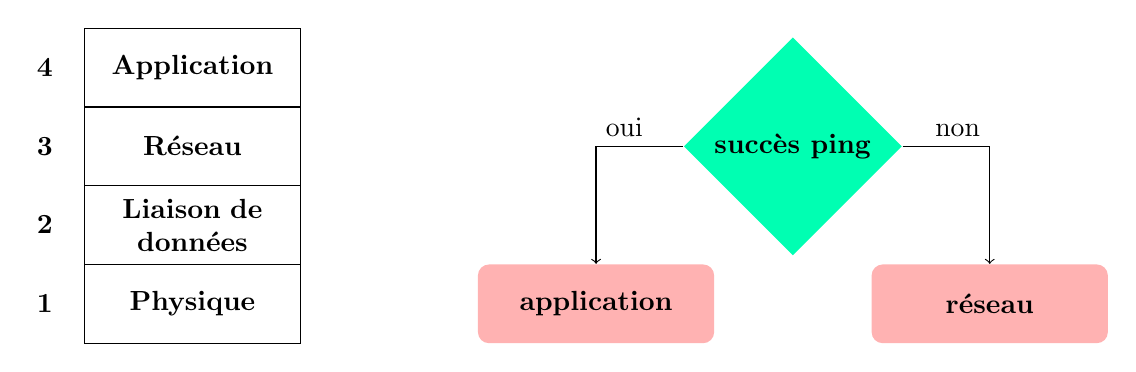
\begin{tikzpicture}
        
        %% Numbers
        \node [minimum height=1cm] at (0,-1) {\textbf{4}};
        \node [minimum height=1cm] at (0,-2) {\textbf{3}};
        \node [minimum height=1cm] at (0,-3) {\textbf{2}};
        \node [minimum height=1cm] at (0,-4) {\textbf{1}};

        %% Rectangles
        \node (application) [anchor=west, text width=2.5cm, text centered, minimum height=1cm, rectangle, draw=black] at (0.5,-1) {\textbf{Application}};
        \node (reseau) [anchor=west, text width=2.5cm, text centered, minimum height=1cm, rectangle, draw=black] at (0.5,-2) {\textbf{Réseau}};
        \node (liaisondonnees) [anchor=west, text width=2.5cm, text centered, minimum height=1cm, rectangle, draw=black] at (0.5,-3) {\textbf{Liaison de données}};
        \node (physique) [anchor=west, text width=2.5cm, text centered, minimum height=1cm, rectangle, draw=black] at (0.5,-4) {\textbf{Physique}};
        
        %% Flowchart
        \node (ping) [choice] at (9.5,-2) {\textbf{succès ping}};
        \node (app)  [root]   at (7,-4)  {\textbf{application}};
        \node (donn) [root]   at (12,-4) {\textbf{réseau}};

        \draw[->] (ping) -| node[anchor=south west]{oui} (app);
        \draw[->] (ping) -| node[anchor=south east]{non} (donn);

    \end{tikzpicture}
\end{center}



\noindent En cas de problème à la fin de la manip:
\begin{enumerate}
    \item Entrer en mode simulation dans Packet Tracer, et essayer de ping entre les machines (\textbf{couche 3}).
    \item Si le ping fonctionne, c'est que le problème vient de la couche application (dhcp, ftp, ssh, etc.).
    \begin{example}
        Exemple -- problème dhcp:
        \begin{enumerate}
            \item filtrer les paquets en fonction du protocole dhcp
            \item vérifier si le paquet a un problème au niveau du serveur ou du relai
        \end{enumerate}
    \end{example}
    \item Si le ping ne fonctionne pas, on vérifie la couche réseau:
    \begin{enumerate}
        \item vérifier la config ip des machines entre lesquelles le ping ne passe pas
        \item vérifier la table de routage (routes statiques \& protocole rip)
        \item vérifier les acl
    \end{enumerate}
    \item Si ça ne fonctionne toujours pas (ou si ça bloque sur un switch), on passe à la couche liaison de données:
    \begin{enumerate}
        \item vérifier que les vlans sont bien configurés
        \item vérifier que la sécurité des ports switchs est configurée correctement
        \item vérifier que la machine trouve bien ses voisins avec le protocole cdp
    \end{enumerate}
    \item A priori, on n'a pas besoin de descendre à la couche physique mais si besoin...
    \begin{enumerate}
        \item vérifier que les machines sont allumées
        \item vérifier que les bonnes interfaces sont allumées
        \item vérifier que les câbles sont branchés aux bonnes interfaces
    \end{enumerate}
\end{enumerate}










\section{Déboguer la configuration réseau en labo -- Approche bottom-up}



\begin{enumerate}
    \item \textcolor{red}{\textbf{Couche physique}} -- Vérifier que le cablâge est correct:
    \begin{enumerate}
        \item regarder si les câbles sont dans les bons ports du routeur (g0/0 ou g0/1)
        \item regarder si les câbles sont branchés dans les bons ports sur les panneaux de brassage
        \item regarder si la couleur des câbles est la bonne (console = bleu, communication = vert)
        \item regarder si le câble est bien branché sur le PC
        \item regarder si le routeur est bien allumé
        \item regarder si une led s'allume sur le routeur quand on branche le câble, \textbf{sinon}, changer le câble
    \end{enumerate}
    \item \textcolor{blue}{\textbf{Couche liaison de données}} -- Vérifier la configuration des cartes réseaux:
    \begin{enumerate}
        \item dans la barre de recherche du pc, taper \texttt{ncpa.cpl}
        \item pour identifier la carte réseau à configurer : débrancher le câble connecté au routeur
        \item rebrancher le câble et configurer la carte réseau où il y a eu le changement
    \end{enumerate}
    \item \textcolor{orange}{\textbf{Couche réseau}} -- Vérifier la configuration IP:
    \begin{enumerate}
        \item utiliser: \texttt{ipconfig}, sur les PC, et: \texttt{show ip interface brief}, sur les routeurs
        \item utiliser: \texttt{show cdp neighbors detail}, pour afficher les ip des machines voisines
        \item utiliser: \texttt{ping}, \texttt{traceroute [-h <max\_nb\_hop>]}, \texttt{tracert [-h <max\_nb\_hop>]}
        \item afficher les routes sur les routeurs, reconfigurer le rip, ou ajouter des routes statiques
    \end{enumerate}
    \item \textcolor{magenta}{\textbf{Couche application}}:
    \begin{enumerate}
        \item désactiver les pare-feux des pc/serveurs
        \item vérifier que le service est bien activé
        \item vérifier que les machines clientes sont bien configurées (pc en dhcp, ip du dns qui correspond)
        \item reconfigurer le dns, dhcp, ftp, etc.
    \end{enumerate}
\end{enumerate}















\part{Annexes}










\section{Problèmes de Packet Tracer}



\begin{itemize}
    \item Impossible d'utiliser: \texttt{login block-for 30 attempts 2 within 120}, sur un switch dans Packet Tracer.
    \item Impossible d'ajouter des adresses IP secondaires dans Packet Tracer.
    \item Impossible d'utiliser la commande: \texttt{load\_helper}, dans Packet Tracer.
    \item Impossible de créer des sous-interfaces sur les interfaces fastethernet dans Packet Tracer.
\end{itemize}










\section{Modes de la console cisco}



\begin{center}
    \begin{tabular}{>{\columncolor{yellow!50}}p{5cm}>{\columncolor{blue!40}}p{7cm}}
        routeur> & exécution utilisateur \\
        routeur\# & exécution privilégiée \\
        routeur(config)\# & configuration (privilégiée) \\
        routeur(config-if)\# & configuration d'interface \\
        routeur(config-router)\# & configuration du protocole de routage \\
        routeur(config-rtr)\# & configuration du protocole de routage ipv6 \\
        routeur(config-line)\# & configuration d'une ligne de terminal \\
        routeur(config-std-nacl)\# & configuration d'une acl standard nommée \\
        routeur(config-ext-nacl)\# & configuration d'une acl étendue nommée \\
        routeur(vlan)\# & création des vlans \\
        routeur(dhcp-config)\# & configuration du service dhcp \\
        rommon 1> & mode rommon (= rom monitor) \\
        switch: & mode rommon (= rom monitor) \\
        switch(config-vlan)\# & configuration de vlan \\
    \end{tabular}
\end{center}










\section{Aides dans le terminal}



\begin{itemize}
    \item \texttt{?} = montre les commandes qui peuvent être utilisé dans le mode actuel
    \item \texttt{<début\_commande>?} = montre les commandes qui commencent par \textit{début\_commande}
    \item \texttt{<commande> ?} = montre les arguments/options que prend la commande
    \item \texttt{<commande>} (sans arguments) = propose des arguments par défaut qui peuvent être modifiés
\end{itemize}
\textbf{Remarques}:
\begin{itemize}
    \item pour certaines commandes (ex: \texttt{copy}), il n'y a pas d'argument par défaut (par contre: \texttt{copy ?}, fonctionne)
    \item \textit{mais}: \texttt{copy flash ftp}, fonctionne, tout comme: \texttt{copy flash running-config}
    \item \texttt{copy flash flash}, ne fonctionne pas
\end{itemize}










\section{Pense-bête VLSM}



\begin{center}
    \begin{tabular}{|p{3.75cm}|p{3.75cm}|p{3.75cm}|p{3.75cm}|} \hline
        \begin{center} \textbf{masque en /} \end{center} &
        \begin{center} \textbf{masque} \end{center} &
        \begin{center} \textbf{wildcard} \end{center} &
        \begin{center} \textbf{nombre d'ip} \end{center}
        \\ \hline
        /1 &  128.0.0.0 & 127.255.255.255 & 2 147 483 648 \\ \hline
        /2 &  192.0.0.0 & 63.255.255.255  & 1 073 741 824 \\ \hline
        /3 &  224.0.0.0 & 31.255.255.255  & 536 870 912 \\ \hline
        /4 &  240.0.0.0 & 15.255.255.255  & 268 435 456 \\ \hline
        /5 &  248.0.0.0 & 7.255.255.255   & 134 217 728 \\ \hline
        /6 &  252.0.0.0 & 3.255.255.255   & 67 108 864 \\ \hline
        /7 &  254.0.0.0 & 1.255.255.255   & 33 554 432 \\ \hline
        /8 &  255.0.0.0 & 0.255.255.255   & 16 777 216 \\ \hline
        /9 &  255.128.0.0 & 0.127.255.255 & 8 388 608 \\ \hline
        /10 & 255.192.0.0 & 0.63.255.255  & 4 194 304 \\ \hline
        /11 & 255.224.0.0 & 0.31.255.255  & 2 097 152 \\ \hline
        /12 & 255.240.0.0 & 0.15.255.255  & 1 048 576 \\ \hline
        /13 & 255.248.0.0 & 0.7.255.255   & 524 288 \\ \hline
        /14 & 255.252.0.0 & 0.3.255.255   & 262 144 \\ \hline
        /15 & 255.254.0.0 & 0.1.255.255   & 131 072 \\ \hline
        /16 & 255.255.0.0 & 0.0.255.255   & 65 536 \\ \hline
        /17 & 255.255.128.0 & 0.0.127.255 & 32 768 \\ \hline
        /18 & 255.255.192.0 & 0.0.63.255  & 16 384 \\ \hline
        /19 & 255.255.224.0 & 0.0.31.255  & 8 192 \\ \hline
        /20 & 255.255.240.0 & 0.0.15.255  & 4 096 \\ \hline
        /21 & 255.255.248.0 & 0.0.7.255   & 2 048 \\ \hline
        /22 & 255.255.252.0 & 0.0.3.255   & 1 024 \\ \hline
        /23 & 255.255.254.0 & 0.0.1.255   & 512 \\ \hline
        /24 & 255.255.255.0 & 0.0.0.255   & 256 \\ \hline
        /25 & 255.255.255.128 & 0.0.0.127 & 128 \\ \hline
        /26 & 255.255.255.192 & 0.0.0.63  & 64 \\ \hline
        /27 & 255.255.255.224 & 0.0.0.31  & 32 \\ \hline
        /28 & 255.255.255.240 & 0.0.0.15  & 16 \\ \hline
        /29 & 255.255.255.248 & 0.0.0.7   & 8 \\ \hline
        /30 & 255.255.255.252 & 0.0.0.3   & 4 \\ \hline
        /31 & 255.255.255.254 & 0.0.0.1   & 2 \\ \hline
        /32 & 255.255.255.255 & 0.0.0.0   & 1 \\ \hline
    \end{tabular}
\end{center}




















\newpage

\tableofcontents





















\end{document}
